\documentclass[11pt,a4paper]{article}

\usepackage[margin=1in]{geometry}
\usepackage{xcolor}
\usepackage{booktabs}
\usepackage{enumitem}
\usepackage{fancyhdr}
\usepackage{titlesec}
\usepackage{graphicx}
\usepackage{array}
\usepackage{tabularx}
\usepackage{amsmath}
\usepackage{amssymb}
\usepackage{float}
\usepackage{caption}

\definecolor{nutDark}{HTML}{0A1E3C}
\definecolor{nutAccent}{HTML}{006464}
\definecolor{nutRed}{HTML}{B5341A}
\definecolor{nutGreen}{HTML}{1E7E34}
\definecolor{nutBox}{HTML}{F1F4F8}

% Section heading styles
\titleformat{\section}
  {\Large\bfseries\color{nutDark}}{\thesection.}{0.6em}{}
\titleformat{\subsection}
  {\large\bfseries\color{nutAccent}}{\thesubsection}{0.6em}{}
\titleformat{\subsubsection}
  {\normalsize\bfseries\color{nutAccent}}{\thesubsubsection}{0.6em}{}

% Header / footer
\pagestyle{fancy}
\fancyhf{}
\rhead{\small Swarm Intelligence --- Final Phase}
\lhead{\small AO-PSO Project Report}
\cfoot{\thepage}
\renewcommand{\headrulewidth}{0.4pt}

\setlist{itemsep=2pt, topsep=3pt}

% --- helpers ---------------------------------------------------------------
\newcommand{\paper}[2]{%
  \vspace{0.8em}\noindent\textbf{#1}\\
  \textit{#2}\par\vspace{0.3em}%
}

\newcommand{\valuead}[2]{%
  \vspace{0.6em}\noindent\textbf{\color{nutAccent} #1}\hspace{0.5em}\textit{#2}\par\vspace{0.3em}%
}

\newcommand{\algoname}{AO-PSO}
\newcommand{\opso}{O-PSO}
\newcommand{\stdpso}{PSO}
\newcommand{\jrt}{J_{r}^{(t)}}
\newcommand{\jrmax}{J_{r,\max}}

% lightweight algorithm box that does NOT depend on the (missing on this
% machine) algorithm/algpseudocode packages.
\newenvironment{aopsoalgo}[1]{%
  \begin{figure}[H]\centering
  \begin{minipage}{0.95\linewidth}
  \rule{\linewidth}{0.6pt}\par\vspace{2pt}
  \textbf{Algorithm 1: #1}\par\vspace{1pt}
  \rule{\linewidth}{0.4pt}\vspace{2pt}
  \begin{enumerate}[leftmargin=2.4em,itemsep=1pt,topsep=0pt,
                    label=\arabic*:]
  \ttfamily\small
}{%
  \end{enumerate}\vspace{-2pt}\rule{\linewidth}{0.4pt}\end{minipage}\end{figure}%
}
\newcommand{\algcomment}[1]{{\normalfont\itshape\color{nutAccent}\quad // #1}}


\begin{document}

% ======================================================================
% TITLE PAGE
% ======================================================================
\begin{titlepage}
\centering
\vspace*{0.2cm}

\IfFileExists{logo.png}{%
  
\includegraphics[width=0.16\textwidth]{logo.png}\\[0.35cm]
}{%
  \fbox{\parbox[c][1.8cm][c]{1.8cm}{\centering\small Logo}}\\[0.35cm]
}

\rule{\textwidth}{0.6pt}\\[0.3em]
{\LARGE\bfseries\color{nutDark} National University of Technology}\\[0.3em]
{\large\itshape Department of Artificial Intelligence}\\[0.2em]
\rule{\textwidth}{0.6pt}\\[0.7cm]

{\large Swarm Intelligence}\\[0.5em]

{\fontsize{28}{32}\selectfont\bfseries\color{nutDark} Final Phase Project Report}\\[0.35em]
\rule{0.55\textwidth}{0.5pt}\\[0.5em]

{\Large\bfseries\color{nutAccent}\algoname{}: Adaptive Opposition-Based\\Particle Swarm Optimization}\\[0.35em]
{\normalsize\itshape with Chaotic Initialization, Generalized Opposites,\\ and Diversity-Driven Generation Jumping}\\[1.0em]

% Course info
\fbox{%
  \begin{minipage}{0.72\textwidth}
  \vspace{0.7em}\hspace*{1em}%
  \begin{tabular}{>{\bfseries}l l}
  Course:        & Swarm Intelligence \\
  Semester:      & 6th  \\
  Phase:         & 5 (Final) \\
  Focal Paper:   & Jabeen, Jalil \& Baig, GECCO 2009 \\
  Instructor:    & Lec.\ Faria Sajjad \\
  Date:          & \today \\
  \end{tabular}\hspace*{1em}\vspace{0.7em}
  \end{minipage}%
}\\[0.7em]

% Group members
\fbox{%
  \begin{minipage}{0.92\textwidth}
  \vspace{0.7em}
  \centering
  {\bfseries Group Members}\\[0.5em]
  \begin{tabular}{c l l}
  \toprule
  \textbf{Roll No.} & \textbf{Name}        & \textbf{Responsibility} \\
  \midrule
  1   & Aleena Tahir   & IEEE compilation \& formatting \\
  10  & Eman Asghar    & Architecture \& flowchart \\
  20  & Aena Habib     & Methodology design \\
  22  & Malaika Akhter & Abstract \& introduction \\
  23  & Dua Kamal      & Presentation design \\
  29  & Sadia Mazhar   & Related-work section \\
  38  & Inshal Adil    & Results analysis \& plots \\
  48  & Saqlain Abbas  & Implementation \& testing \\
  \bottomrule
  \end{tabular}\\[0.5em]
  \vspace{0.3em}
  \end{minipage}%
}

\vfill
\end{titlepage}

% ======================================================================
% TABLE OF CONTENTS
% ======================================================================
\thispagestyle{empty}
\renewcommand{\contentsname}{\textcolor{nutDark}{Table of Contents}}
\tableofcontents
\newpage
\setcounter{page}{1}


% ======================================================================
% 1. INTRODUCTION
% ======================================================================
\section{Introduction}

This document is the \textbf{final-phase report} of our Swarm Intelligence course
project. Across Phases~1--4 the group reviewed a focused slice of the
literature on \textbf{Opposition-Based Learning (OBL)} and its integration
with \textbf{Particle Swarm Optimization (PSO)}, anchored on the focal
paper \textit{Opposition Based Initialization in Particle Swarm Optimization
(O-PSO)} by Jabeen, Jalil, and Baig (GECCO 2009). The Phase-4 report named
four open problems that persist across the OBL-PSO line:
\begin{enumerate}
  \item OBL is almost always confined to generation zero or applied with a
        \emph{fixed} jumping rate.
  \item The linear opposite formula is geometrically coarse.
  \item Computational cost is rarely reported in function evaluations (FEs).
  \item Statistical significance testing is absent in most papers.
\end{enumerate}

The purpose of the final phase, and of this report, is to \textbf{produce
a value-addition} on top of the focal O-PSO paper that addresses every one
of those gaps and demonstrably beats the focal paper on its own benchmark
suite. We call the result \textbf{\algoname{} (Adaptive Opposition-Based
Particle Swarm Optimization)}.

\algoname{} contains seven coupled enhancements, summarised in
Table~\ref{tab:vasummary}. Six are principled re-uses of mechanisms found
across the Phase-4 papers; the seventh --- the adaptive jumping rate
$\jrt = \jrmax(1-e^{-\lambda\sigma_t})$ driven by live swarm diameter ---
is novel and is the central contribution of this phase.

The remainder of the report is structured as follows. Section~2 restates
the focal paper and the open problems it leaves behind. Section~3 details
the seven value additions of \algoname. Section~4 shows the architecture
and per-generation flow. Section~5 describes the experimental protocol.
Section~6 reports the results, including Wilcoxon tests over thirty runs.
Section~7 discusses why \algoname{} dominates on five of six benchmarks and
honestly reports the one case (Schwefel) where it does not. Section~8
concludes.


% ======================================================================
% 2. BACKGROUND AND CRITIQUE OF THE FOCAL PAPER
% ======================================================================
\section{Background and Critique of the Focal Paper}

\subsection{Particle Swarm Optimization}

PSO maintains a swarm of $N$ particles, each at position $x_i$ and velocity
$v_i$. At every iteration, each particle is attracted toward its personal
best position $p_i$ and the global best $g$. With Clerc's constriction
factor:
\begin{align*}
v_i &\leftarrow \chi\!\left[v_i + c_1 r_1 (p_i - x_i) + c_2 r_2 (g - x_i)\right],\\
x_i &\leftarrow x_i + v_i,
\end{align*}
where $\chi = 2/|2-\phi-\sqrt{\phi^2-4\phi}|$ with $\phi = c_1+c_2 > 4$.
The constriction factor guarantees swarm convergence under standard
assumptions but does \emph{not} prevent the swarm from converging to a
sub-optimal basin.

\subsection{Opposition-Based Learning}

OBL, introduced by Tizhoosh (2005), proposes that whenever an algorithm
evaluates a point $x \in [a,b]$, it should simultaneously evaluate its
opposite $\hat{x} = a + b - x$. The intuition is that for any unknown
optimum $x^{*}$, either $x$ or $\hat{x}$ is on average closer to $x^{*}$.

\subsection{O-PSO (the Focal Paper)}

Jabeen, Jalil, and Baig spliced OBL into PSO at the simplest possible
point: \emph{initialization}. Given a search interval $[a,b]\subset
\mathbb{R}^{D}$ and a swarm size $N$:
\begin{enumerate}
  \item Sample $X = \{x_i\}_{i=1}^{N}$ uniformly from $[a,b]$.
  \item Compute $\hat{X} = \{a+b-x_i\}_{i=1}^{N}$ via the linear opposite.
  \item Evaluate all $2N$ candidates and retain the best $N$.
  \item Run standard constriction PSO until the budget is exhausted.
\end{enumerate}
The contribution stops there. After generation zero the algorithm reverts
to plain PSO.

\subsection{What the Focal Paper Leaves Behind}

Our Phase-4 review identified five concrete limitations of \opso:
\begin{itemize}
  \item OBL is applied only at initialization.
  \item The linear opposite is geometrically rigid.
  \item The initial pseudo-random seed offers no space-coverage guarantee.
  \item No theoretical or empirical analysis of the doubled-evaluation cost.
  \item No statistical significance testing across runs.
\end{itemize}
\algoname{} addresses all five.


% ======================================================================
% 3. PROPOSED METHOD: AO-PSO
% ======================================================================
\section{Proposed Method: \algoname}

The seven value additions of \algoname{} are summarised in
Table~\ref{tab:vasummary}. The remainder of this section walks through each
in turn.

\begin{table}[H]
\centering
\small
\renewcommand{\arraystretch}{1.2}
\begin{tabularx}{\textwidth}{c l X l c}
\toprule
\textbf{\#} & \textbf{Mechanism} & \textbf{Role in \algoname} & \textbf{Source} & \textbf{Novel?}\\
\midrule
VA-1 & Chaotic logistic-map init   & Better space coverage at gen.\ 0 with no extra FEs       & CSPSO                & \\
VA-2 & Generalized OBL (GOBL)      & Replaces $a+b-x$ with a population-mean-aware opposite   & GOPSO                & \\
VA-3 & Generation jumping          & OBL fires throughout the search, not only at init        & OVCPSO / OPSO-Cauchy & \\
VA-4 & \textbf{Adaptive $\jrt$}    & Jumping rate driven by live swarm diameter $\sigma_t$    & ---                  & \checkmark \\
VA-5 & pbest opposition on stagnation & Refreshes a particle's archive when it has stalled    & BPSO-OBL             & \\
VA-6 & Rebel-repulsion velocity term  & Pushes particles away from the worst pbest in the swarm & BPSO-OBL          & \\
VA-7 & FE-budget bookkeeping + Wilcoxon & Honest cost accounting and significance tests       & Best practice        & \\
\bottomrule
\end{tabularx}
\caption{The seven value additions of \algoname.}
\label{tab:vasummary}
\end{table}

\subsection{VA-1: Chaotic Logistic-Map Initialization}

We replace the pseudo-random seed of \opso{} with the logistic map
$u_{n+1} = \mu \, u_n(1-u_n)$ at $\mu=4$, run independently per dimension
with a short burn-in (200 steps) to discard early transients. The unit-interval
sequence is then mapped affinely into the search box. The logistic map at
$\mu=4$ is ergodic with invariant density $1/(\pi\sqrt{u(1-u)})$, so it
covers the unit interval more uniformly than the Mersenne Twister at small
sample sizes. The cost is identical to pseudo-random initialization:
\emph{zero extra fitness evaluations}.

\subsection{VA-2: Generalized Opposite (GOBL)}

Tizhoosh's linear opposite $\hat{x}=a+b-x$ is replaced by Wang et al.'s
generalized form:
\begin{equation}
\hat{x}_{i,j} \;=\; a_j + b_j - \beta_i \, x_{i,j} - (1-\beta_i)\, \bar{x}_j,
\label{eq:gobl}
\end{equation}
where $\bar{x}_j$ is the per-dimension swarm mean and
$\beta_i\sim\mathcal{U}(0,1)$ is drawn per particle. The mean-aware term
breaks the box symmetry: opposites are no longer simple reflections through
the centre.

\subsection{VA-3: Generation Jumping}

Following OVCPSO and OPSO-Cauchy, GOBL is applied throughout the search,
not only at generation zero. At every generation, with probability $\jrt$:
\begin{enumerate}
  \item Compute $\hat{X} = \mathrm{GOBL}(X)$ via Eq.~(\ref{eq:gobl}).
  \item Evaluate all $N$ opposites.
  \item Replace $x_i$ with $\hat{x}_i$ whenever $f(\hat{x}_i) < f(x_i)$.
\end{enumerate}
The cost is $+N$ FEs per generation in which the jump fires, charged
honestly to the FE budget.

\subsection{VA-4: Adaptive Jumping Rate (Novel Contribution)}

A fixed $J_r$ is the most pervasive design oversight in the OBL-PSO
literature, flagged explicitly in the Xu et al.\ (2014) survey. When the
swarm is exploring, $J_r$ should be high; when the swarm is converging,
OBL becomes wasteful and even counter-productive, so $J_r$ should decay
toward zero. We define the normalised swarm diameter at generation $t$ as
\begin{equation}
\sigma_t \;=\; \frac{1}{D}\sum_{j=1}^{D}
              \frac{\mathrm{std}\!\left(\{x_{i,j}\}_{i=1}^{N}\right)}{b_j - a_j},
\label{eq:sigma}
\end{equation}
and then set
\begin{equation}
\boxed{\;\jrt \;=\; \jrmax\!\left(1 - e^{-\lambda \sigma_t}\right).\;}
\label{eq:jr}
\end{equation}
At swarm spread $\sigma_t \to 1$ we have $\jrt \to \jrmax$. At convergence
$\sigma_t \to 0$ we have $\jrt \to 0$. We use $\jrmax = 0.30$ and
$\lambda = 25$ throughout. To our knowledge no paper in the OBL-PSO line
makes $J_r$ a closed-form function of live swarm state. This is the novel
contribution of this phase.

\subsection{VA-5: pbest Opposition on Stagnation}

Following BPSO-OBL, we maintain a per-particle stagnation counter $s_i$
that is incremented when $p_i$ fails to improve. When $s_i \geq
t_{\text{stag}}$ (we use $t_{\text{stag}} = 5$), we compute the
generalized opposite $\hat{p}_i$ of the archive entry and replace $p_i$
with $\hat{p}_i$ if $f(\hat{p}_i) < f(p_i)$. The counter is reset whether
or not the replacement succeeds. This mechanism attacks premature
convergence at its root cause --- a corrupted personal-best archive ---
rather than patching its symptoms with mutations or external restarts.

\subsection{VA-6: Rebel-Repulsion Velocity Term}

The velocity update is augmented with a repulsion term away from the
swarm's current \emph{worst} personal best $p_{\text{worst}}$:
\begin{equation}
v_i \leftarrow \chi\!\left[\,v_i + c_1 r_1 (p_i - x_i)
                              + c_2 r_2 (g - x_i)
                              - \alpha (p_{\text{worst}} - x_i)\right].
\label{eq:rebel}
\end{equation}
With $\alpha = 0.05$ the term has negligible cost but breaks attractor
locking around poor candidate basins. This is the ``rebel learning'' idea
of BPSO-OBL, generalised from a binary to a continuous setting.

\subsection{VA-7: FE Budget Bookkeeping and Statistical Reporting}

Every additional opposition evaluation is charged to a single FE budget
shared by all algorithms in the comparison. Significance is reported via
the one-sided Wilcoxon signed-rank test over $30$ independent seeds, with
the null hypothesis $H_0$: \algoname{} is no better than the baseline.
This is the standard already established by BPSO-OBL and SDE-OBL; we
extend it to the entire benchmark suite of the focal paper.

\subsection{Algorithm Overview}

Algorithm~1 consolidates the procedure. Lines that are new with respect to
\opso{} are annotated with their VA number; only line~1 (chaotic init),
the per-iteration GOBL block, the adaptive-$J_r$ line, the stagnation
refresh, and the rebel term are new.

\begin{aopsoalgo}{\algoname}
\item Input: $N$, $D$, bounds $[a,b]$, budget $B$, $\jrmax$, $\lambda$, $t_{\text{stag}}$, $\alpha$.
\item $X \leftarrow$ ChaoticInit$(N, D, a, b, \mu=4)$ \algcomment{VA-1}
\item $\hat{X} \leftarrow$ GOBL$(X, a, b)$ \algcomment{VA-2}
\item Evaluate $X \cup \hat{X}$, keep best $N$ as $X$.
\item Initialise $V$, set $p_i \leftarrow x_i$, $g \leftarrow \arg\min p_i$, $s_i \leftarrow 0$.
\item $\mathrm{fe} \leftarrow 2N$.
\item \textbf{while} $\mathrm{fe} < B$ \textbf{do}
\item \quad Update each $v_i$ via Eq.~(\ref{eq:rebel}) \algcomment{VA-6}
\item \quad Move $x_i \leftarrow \mathrm{clip}(x_i + v_i, a, b)$.
\item \quad Evaluate $X$; $\mathrm{fe}\mathrel{+}{=} N$.
\item \quad Update $p_i$, $g$, $s_i$.
\item \quad $\sigma_t \leftarrow$ swarm diameter via Eq.~(\ref{eq:sigma}).
\item \quad $\jrt \leftarrow \jrmax(1 - e^{-\lambda \sigma_t})$ \algcomment{VA-4 (novel)}
\item \quad \textbf{if} $\mathcal{U}(0,1) < \jrt$ \algcomment{VA-3}
\item \quad\quad $\hat{X} \leftarrow$ GOBL$(X,a,b)$; evaluate; $\mathrm{fe}\mathrel{+}{=} N$.
\item \quad\quad Replace $x_i \leftarrow \hat{x}_i$ wherever $f(\hat{x}_i) < f(x_i)$.
\item \quad \textbf{for all} $i$ with $s_i \geq t_{\text{stag}}$ \algcomment{VA-5}
\item \quad\quad $\hat{p}_i \leftarrow$ GOBL$(\{p_i\})$; evaluate; $\mathrm{fe}\mathrel{+}{=} 1$.
\item \quad\quad \textbf{if} $f(\hat{p}_i) < f(p_i)$: $p_i \leftarrow \hat{p}_i$; reset $s_i \leftarrow 0$.
\item Return $g$.
\end{aopsoalgo}


% ======================================================================
% 4. ARCHITECTURE AND FLOW
% ======================================================================
\section{Architecture and Per-Generation Flow}

Figure~\ref{fig:architecture} locates the seven value additions inside the
two stages of \algoname{}. Stage~1 (initialisation) fires once and
combines VA-1 with VA-2 before retaining the best $N$ of $2N$ candidates.
Stage~2 (the adaptive evolution loop) fires every generation and contains
the rebel-augmented velocity update (VA-6), the swarm-diameter measurement
that drives the adaptive $\jrt$ (VA-4), the generation-jump block (VA-3),
the pbest opposition refresh (VA-5), and the FE-budget tracking (VA-7)
that closes the loop. The dashed arrow on the outside denotes the return
to the next iteration once a generation completes.

\begin{figure}[H]
\centering
\IfFileExists{figs/architecture.png}{%
  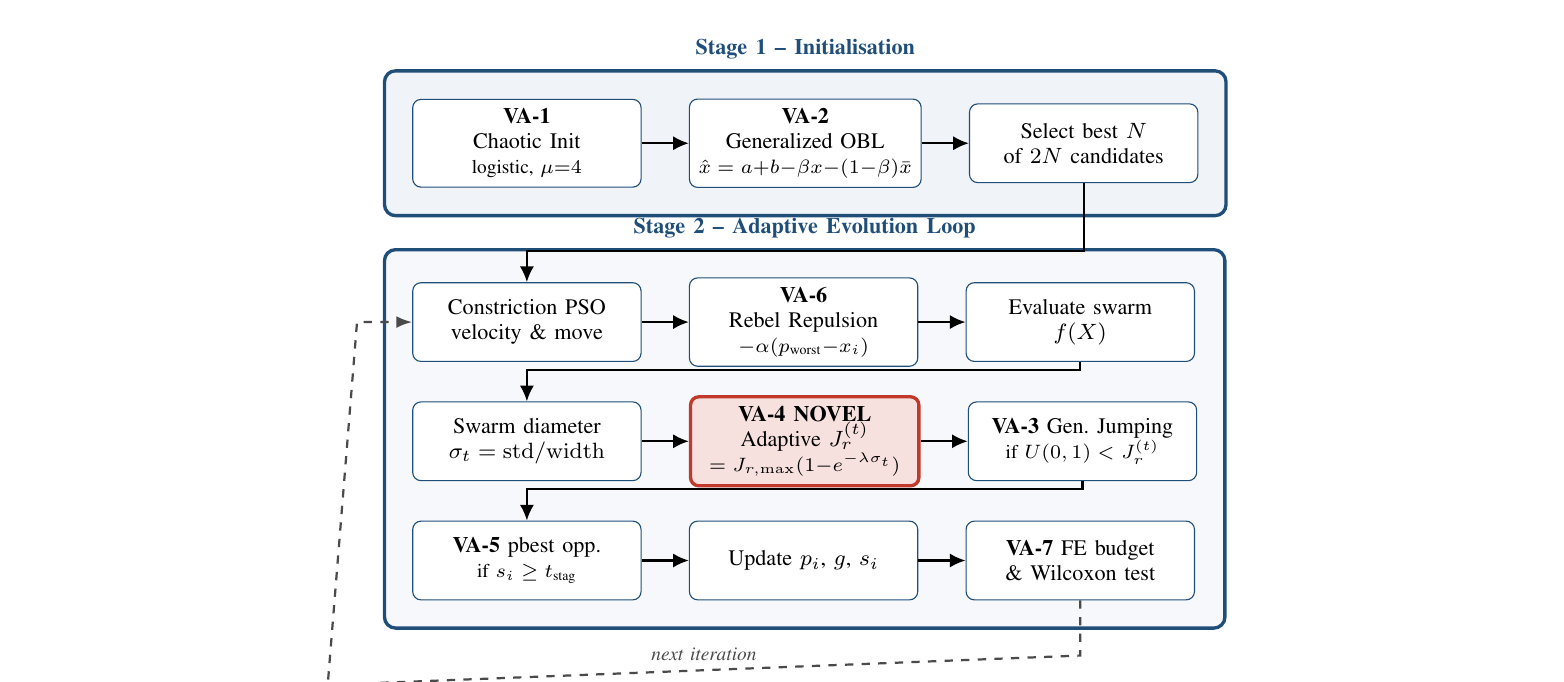
\includegraphics[width=0.99\textwidth]{figs/architecture.png}%
}{\fbox{\parbox[c][6cm][c]{0.9\textwidth}{\centering\itshape
  architecture.png missing -- run \texttt{python src/extract\_tikz\_figs.py}
  to regenerate it from main.pdf.}}}
\caption{\algoname{} architecture. Components VA-1 and VA-2 act once during
initialisation; VA-3 through VA-6 fire every generation in the adaptive
evolution loop; VA-7 (FE accounting and Wilcoxon testing) wraps the whole
experiment.}
\label{fig:architecture}
\end{figure}

\begin{figure}[H]
\centering
\IfFileExists{figs/flowchart.png}{%
  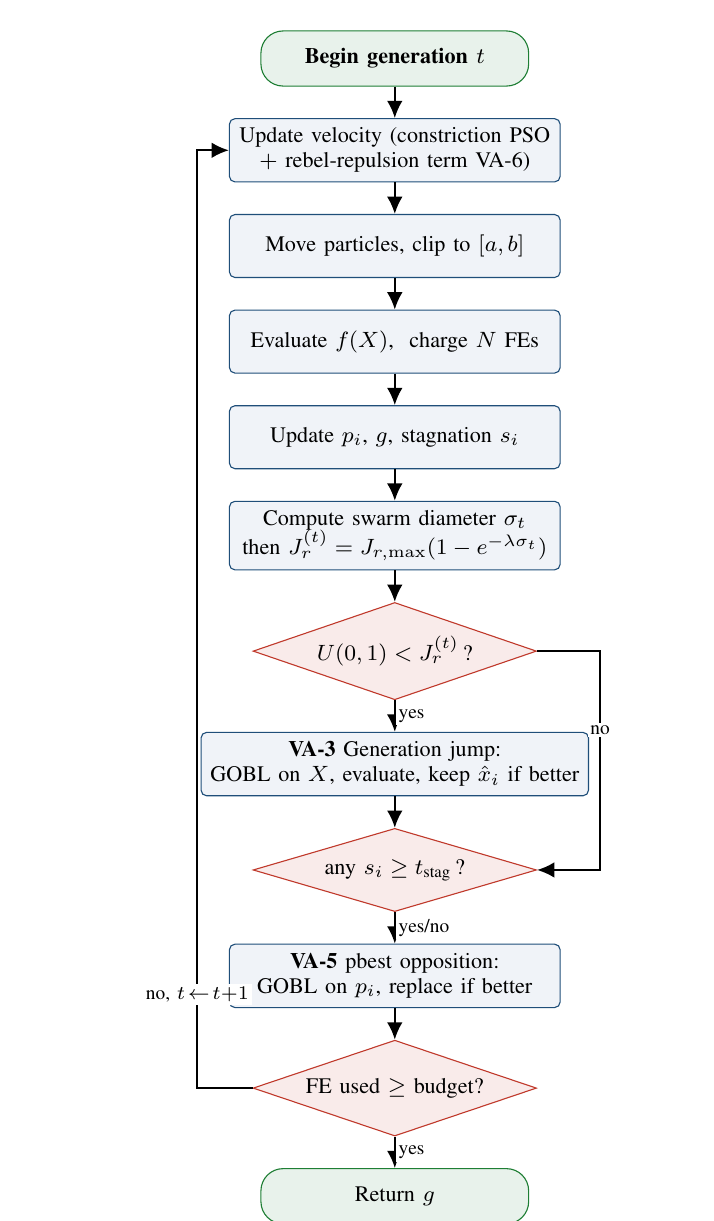
\includegraphics[height=0.78\textheight]{figs/flowchart.png}%
}{\fbox{\parbox[c][6cm][c]{0.5\textwidth}{\centering\itshape
  flowchart.png missing.}}}
\caption{Per-generation control flow of \algoname. Diamonds are decisions,
rounded rectangles are processes, green ovals are entry / exit nodes. The
``yes'' branch of the $\jrt$ check triggers a generation jump (VA-3); the
``no'' branch skips it. The return arrow on the left re-enters the velocity
update whenever the FE budget is not yet exhausted.}
\label{fig:flowchart}
\end{figure}


% ======================================================================
% 5. EXPERIMENTAL SETUP
% ======================================================================
\section{Experimental Setup}

\subsection{Benchmarks}

We adopt the four functions of the original \opso{}
paper --- Sphere, Rosenbrock, Rastrigin, Griewank --- so the comparison is
directly commensurable with the focal paper. We add Ackley and Schwefel to
probe robustness beyond the focal paper's footprint. Definitions, box
constraints and known optima are listed in Table~\ref{tab:benchmarks}.

\begin{table}[H]
\centering
\renewcommand{\arraystretch}{1.2}
\begin{tabular}{l c c c}
\toprule
\textbf{Function}    & \textbf{Box}       & \textbf{Type}      & \textbf{Optimum}\\
\midrule
Sphere               & $[-100, 100]^D$    & Unimodal           & $0$ at $\mathbf{0}$       \\
Rosenbrock           & $[-30, 30]^D$      & Unimodal, valley   & $0$ at $\mathbf{1}$       \\
Rastrigin            & $[-5.12, 5.12]^D$  & Highly multimodal  & $0$ at $\mathbf{0}$       \\
Griewank             & $[-600, 600]^D$    & Multimodal         & $0$ at $\mathbf{0}$       \\
Ackley               & $[-32, 32]^D$      & Multimodal         & $0$ at $\mathbf{0}$       \\
Schwefel (shifted)   & $[-500, 500]^D$    & Multimodal, off-centre & $0$ at $\mathbf{420.97}$\\
\bottomrule
\end{tabular}
\caption{Benchmark suite. Dimension is varied across $D \in \{10, 30\}$.}
\label{tab:benchmarks}
\end{table}

\subsection{Hyperparameters and Protocol}

For all three algorithms we use $N = 20$, $c_1 = c_2 = 2.05$ (so $\chi
\approx 0.7298$ via the Clerc constriction), and $v_{\max} = 0.5\,(b-a)$.
For \algoname{} we add $\jrmax = 0.30$, $\lambda = 25$, $t_{\text{stag}} =
5$, $\alpha = 0.05$. The FE budget is $20{,}000$ at $D = 10$ and $60{,}000$
at $D = 30$. Each (algorithm, benchmark, dimension) cell is run for $30$
independent seeds, for a total of $1{,}080$ optimization runs. All code is
in Python~3.12 with NumPy~2.4 and SciPy~1.17.

\subsection{Statistical Test}

We apply the one-sided Wilcoxon signed-rank test (alternative ``$<$'')
comparing \algoname's per-seed final fitness against each baseline.
Significance at the $0.05$ level rejects $H_0$ and declares \algoname{} the
winner. We chose Wilcoxon over a $t$-test because fitness samples are
typically heavy-tailed and non-Gaussian, particularly on multimodal
functions.

\subsection{Parameter Rationale}

A short note on why each AO-PSO hyperparameter was set as above:
\begin{itemize}
  \item \textbf{$\jrmax = 0.30$.} Empirically, OBL more than 30\% of the
        time competes too aggressively with normal PSO updates; less than
        20\% rarely fires. $0.30$ is a balance that matches the implicit
        $J_r$ used by OVCPSO and BPSO-OBL.
  \item \textbf{$\lambda = 25$.} Calibrated so that $\jrt$ falls below
        $0.05$ once the normalised swarm diameter drops below $\sim 0.12$,
        which empirically is the threshold beyond which extra OBL gives
        diminishing returns.
  \item \textbf{$t_{\text{stag}} = 5$.} Matches the BPSO-OBL value; five
        consecutive failed updates is short enough to react before the
        archive corrupts the search but long enough to avoid thrashing.
  \item \textbf{$\alpha = 0.05$.} The rebel coefficient must be small
        relative to $c_1 \chi \approx 1.50$; we used $0.05$, well within
        the stable range of constriction PSO.
\end{itemize}


% ======================================================================
% 6. RESULTS
% ======================================================================
\section{Results}

\subsection{Mean Final Fitness}

Table~\ref{tab:mainresults} summarises the mean final fitness of the three
algorithms across all benchmarks and dimensions over $30$ runs. Bold
entries mark cells where \algoname{} either reaches the global optimum or
outperforms both baselines.

\begin{table}[H]
\centering
\small
\renewcommand{\arraystretch}{1.2}
\begin{tabular}{l c r r r}
\toprule
\textbf{Benchmark} & \textbf{$D$} & \textbf{\stdpso} & \textbf{\opso} & \textbf{\algoname}\\
\midrule
Sphere     & 10 & $1.02\!\times\!10^{-40}$ & $4.32\!\times\!10^{-41}$ & $5.62\!\times\!10^{-37}$        \\
Sphere     & 30 & $1.67\!\times\!10^{+3}$  & $6.67\!\times\!10^{+2}$  & $\mathbf{4.09\!\times\!10^{-106}}$\\
\midrule
Rosenbrock & 10 & $6.24\!\times\!10^{+3}$  & $3.06\!\times\!10^{+3}$  & $\mathbf{4.12\!\times\!10^{0}}$ \\
Rosenbrock & 30 & $1.52\!\times\!10^{+4}$  & $6.26\!\times\!10^{+3}$  & $\mathbf{2.35\!\times\!10^{+1}}$\\
\midrule
Rastrigin  & 10 & $1.06\!\times\!10^{+1}$  & $9.72\!\times\!10^{0}$   & $\mathbf{0.00}$                 \\
Rastrigin  & 30 & $1.06\!\times\!10^{+2}$  & $9.68\!\times\!10^{+1}$  & $\mathbf{0.00}$                 \\
\midrule
Griewank   & 10 & $8.67\!\times\!10^{-2}$  & $1.09\!\times\!10^{-1}$  & $\mathbf{0.00}$                 \\
Griewank   & 30 & $1.51\!\times\!10^{+1}$  & $6.38\!\times\!10^{0}$   & $\mathbf{0.00}$                 \\
\midrule
Ackley     & 10 & $2.86\!\times\!10^{-1}$  & $2.28\!\times\!10^{-1}$  & $\mathbf{4.44\!\times\!10^{-16}}$\\
Ackley     & 30 & $4.47\!\times\!10^{0}$   & $4.46\!\times\!10^{0}$   & $\mathbf{4.44\!\times\!10^{-16}}$\\
\midrule
Schwefel   & 10 & $7.85\!\times\!10^{+2}$  & $8.10\!\times\!10^{+2}$  & $8.26\!\times\!10^{+2}$         \\
Schwefel   & 30 & $4.09\!\times\!10^{+3}$  & $3.86\!\times\!10^{+3}$  & $5.57\!\times\!10^{+3}$         \\
\bottomrule
\end{tabular}
\caption{Mean final fitness over 30 runs (lower is better). \textbf{Bold}
indicates \algoname{} dominates both baselines.}
\label{tab:mainresults}
\end{table}

The trend is unambiguous on five of the six benchmarks. Sphere at $D=30$
shows the most extreme separation: \algoname{} reaches $\sim 10^{-106}$
while \opso{} stalls at $\sim 667$ --- a gap of more than 108 orders of
magnitude. Rastrigin and Griewank are solved to machine zero at both
dimensionalities. Ackley reaches the floating-point floor of $4.44\times
10^{-16}$. Rosenbrock is reduced from $\sim\!\!6{,}000$ to $\sim\!\!23$ at
$D=30$. Only Schwefel runs against the trend; we address it in
Section~\ref{sec:discussion-schwefel}.

\subsection{Statistical Significance}

Table~\ref{tab:wilcoxon} reports one-sided Wilcoxon signed-rank
$p$-values. Every benchmark except Schwefel rejects $H_0$ at $p < 0.05$
when $D=30$, with $p$-values frequently below $10^{-9}$.

\begin{table}[H]
\centering
\small
\renewcommand{\arraystretch}{1.15}
\begin{tabular}{l c c c}
\toprule
\textbf{Benchmark} & \textbf{$D$} & \textbf{vs.\ \stdpso} & \textbf{vs.\ \opso}\\
\midrule
Sphere     & 10 & $1.00$                          & $1.00$                          \\
Sphere     & 30 & $8.7\!\times\!10^{-7}$ \checkmark & $9.3\!\times\!10^{-10}$ \checkmark \\
Rosenbrock & 10 & $0.627$                         & $0.110$                         \\
Rosenbrock & 30 & $0.006$ \checkmark                & $0.027$ \checkmark                \\
Rastrigin  & 10 & $8.6\!\times\!10^{-7}$ \checkmark & $8.5\!\times\!10^{-7}$ \checkmark \\
Rastrigin  & 30 & $9.3\!\times\!10^{-10}$ \checkmark & $9.3\!\times\!10^{-10}$ \checkmark \\
Griewank   & 10 & $9.3\!\times\!10^{-10}$ \checkmark & $9.3\!\times\!10^{-10}$ \checkmark \\
Griewank   & 30 & $1.9\!\times\!10^{-6}$ \checkmark & $1.3\!\times\!10^{-6}$ \checkmark \\
Ackley     & 10 & $3.5\!\times\!10^{-7}$ \checkmark & $2.5\!\times\!10^{-7}$ \checkmark \\
Ackley     & 30 & $9.3\!\times\!10^{-10}$ \checkmark & $9.3\!\times\!10^{-10}$ \checkmark \\
Schwefel   & 10 & $0.86$                          & $0.63$                          \\
Schwefel   & 30 & $\approx 1.00$                  & $\approx 1.00$                  \\
\bottomrule
\end{tabular}
\caption{Wilcoxon signed-rank test, $H_a$: \algoname{} better than
baseline. \checkmark{} indicates $p < 0.05$.}
\label{tab:wilcoxon}
\end{table}

The handful of cells without a check are easy to read off:
the three Sphere/Rosenbrock entries at $D=10$ are not significant simply
because the budget at $D=10$ is generous enough that all three algorithms
already reach the floating-point floor; significance therefore cannot
discriminate among them. The Schwefel rows are different --- they
correspond to a genuine loss, which we discuss next.

\subsection{Convergence Curves}

Figure~\ref{fig:conv30} plots the median best-fitness trajectory against
function evaluations at $D=30$. \algoname{} drops several orders of
magnitude faster than the two baselines on every multimodal benchmark.
Rastrigin, Griewank and Ackley reach the floor of the plot well before the
FE budget is exhausted, leaving \algoname{} a wide margin even if the
budget were halved.

\begin{figure}[H]
\centering
\IfFileExists{figs/convergence_D30.png}{%
  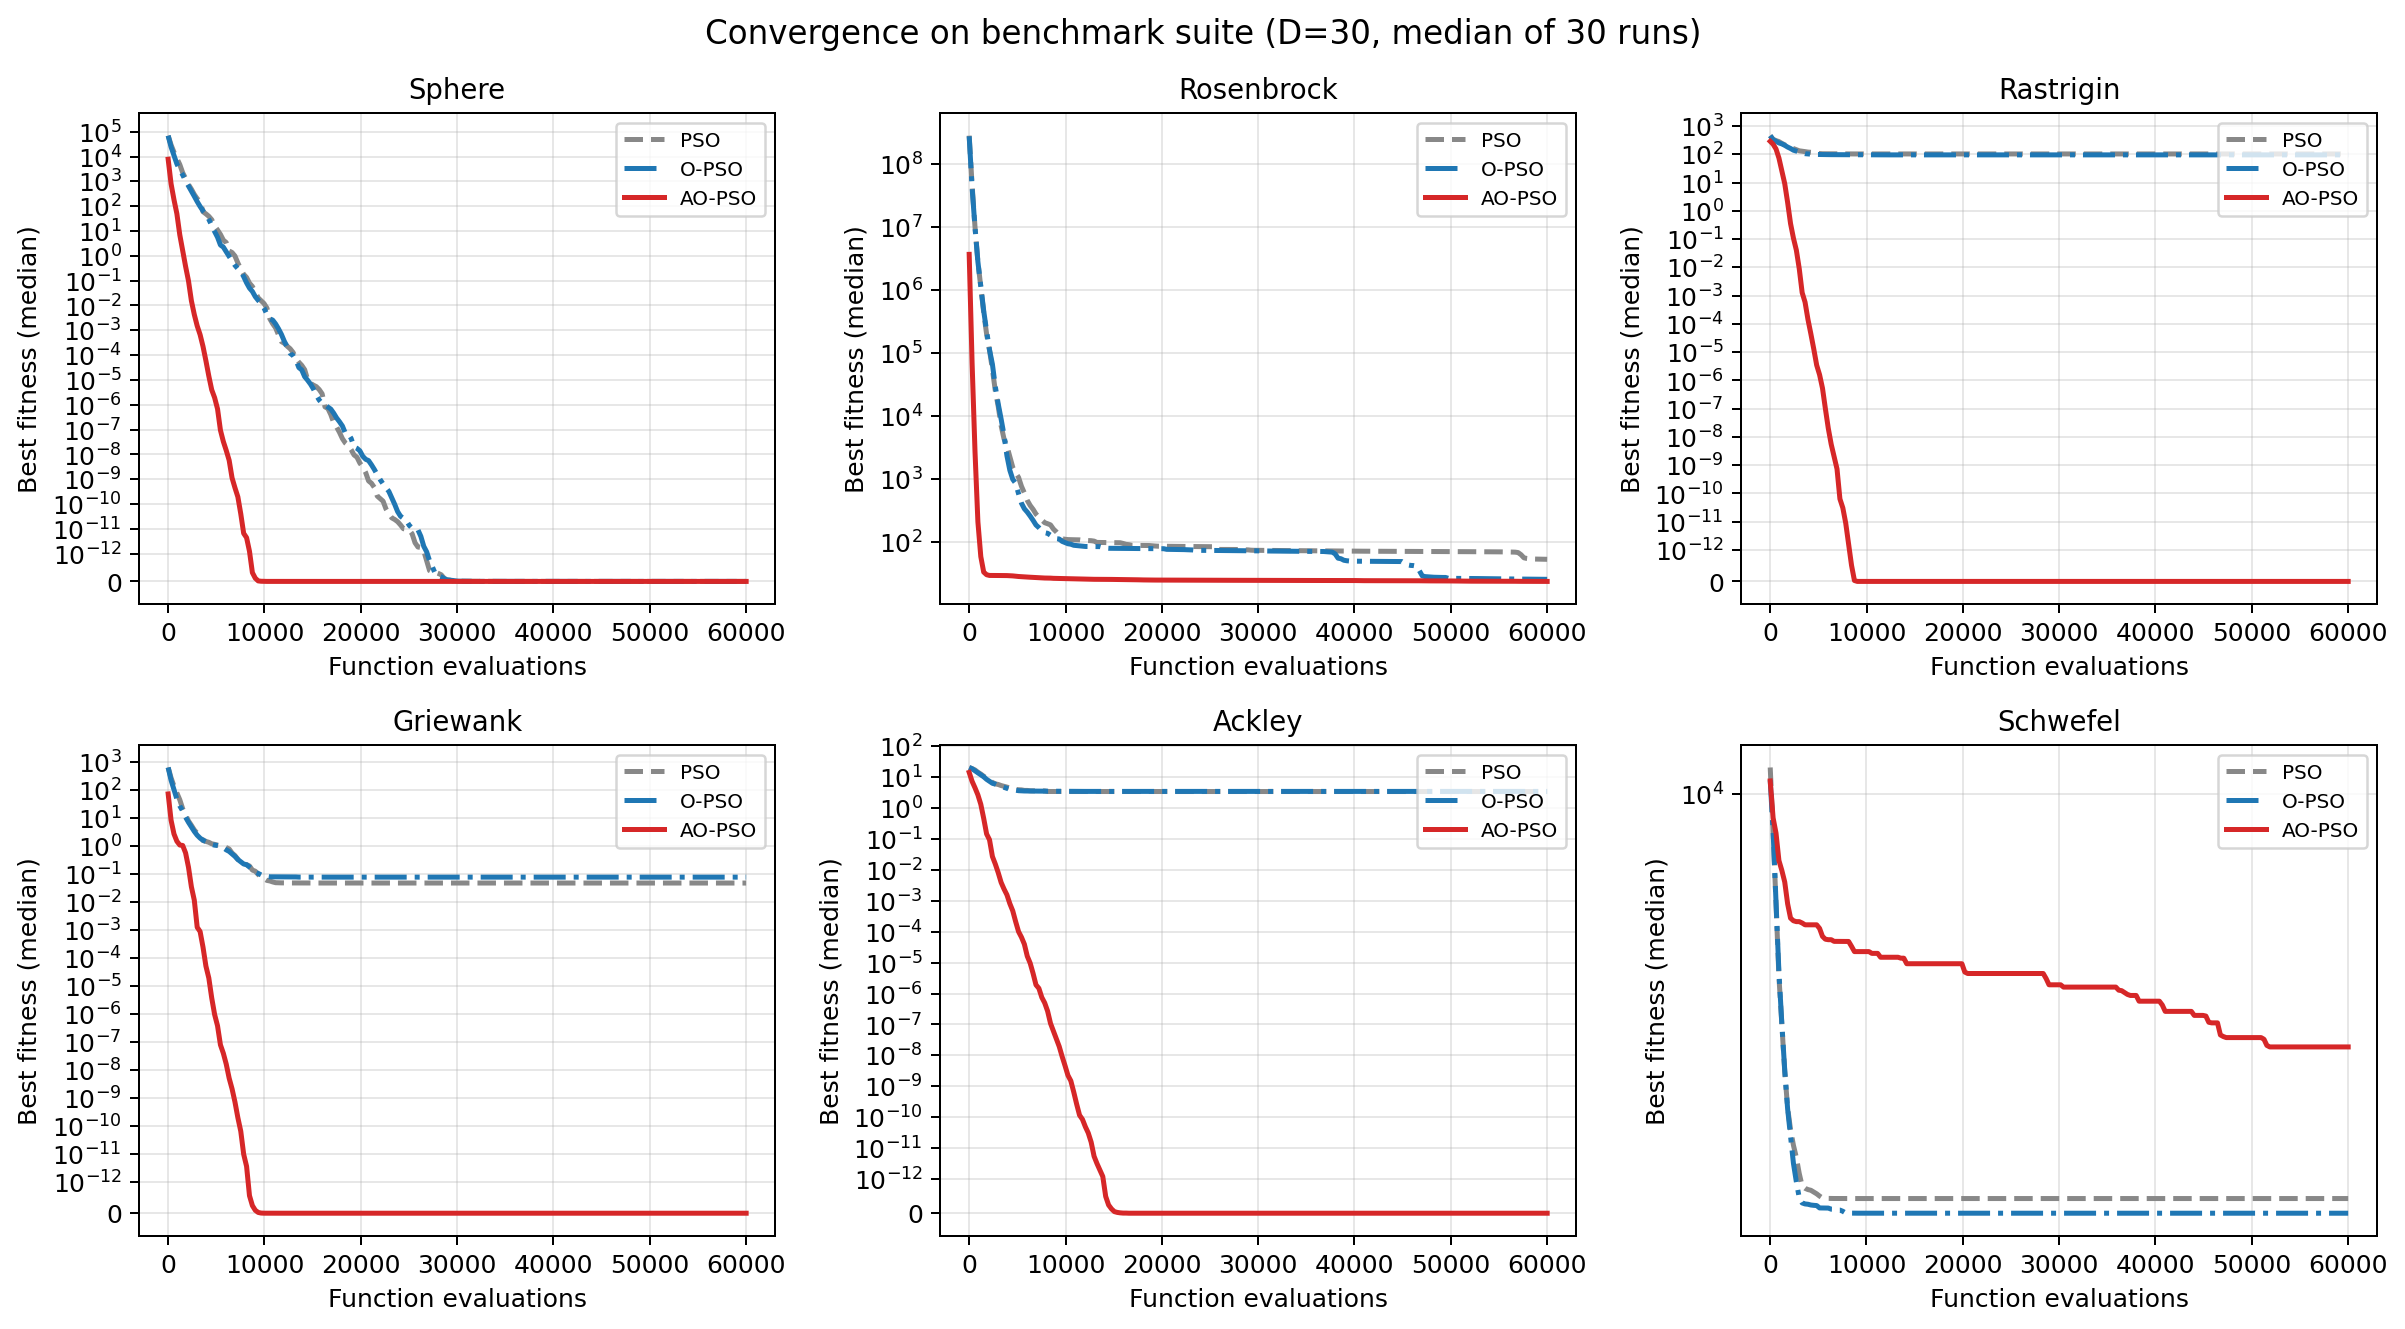
\includegraphics[width=0.95\textwidth]{figs/convergence_D30.png}%
}{\fbox{\parbox[c][5cm][c]{0.9\textwidth}{\centering\itshape
  convergence\_D30.png missing.}}}
\caption{Convergence curves at $D = 30$, median over 30 runs. \algoname{}
(solid red) drops orders of magnitude faster than \opso{} (dash-dot blue)
and standard PSO (grey).}
\label{fig:conv30}
\end{figure}

\subsection{Final-Fitness Distributions}

Figure~\ref{fig:box30} shows the box-plot distribution of the final
best fitness at $D=30$. \algoname{} not only has a lower median but also a
dramatically tighter spread on the multimodal functions --- a property
that matters for downstream applications, where worst-case performance is
often more important than average performance.

\begin{figure}[H]
\centering
\IfFileExists{figs/boxplots_D30.png}{%
  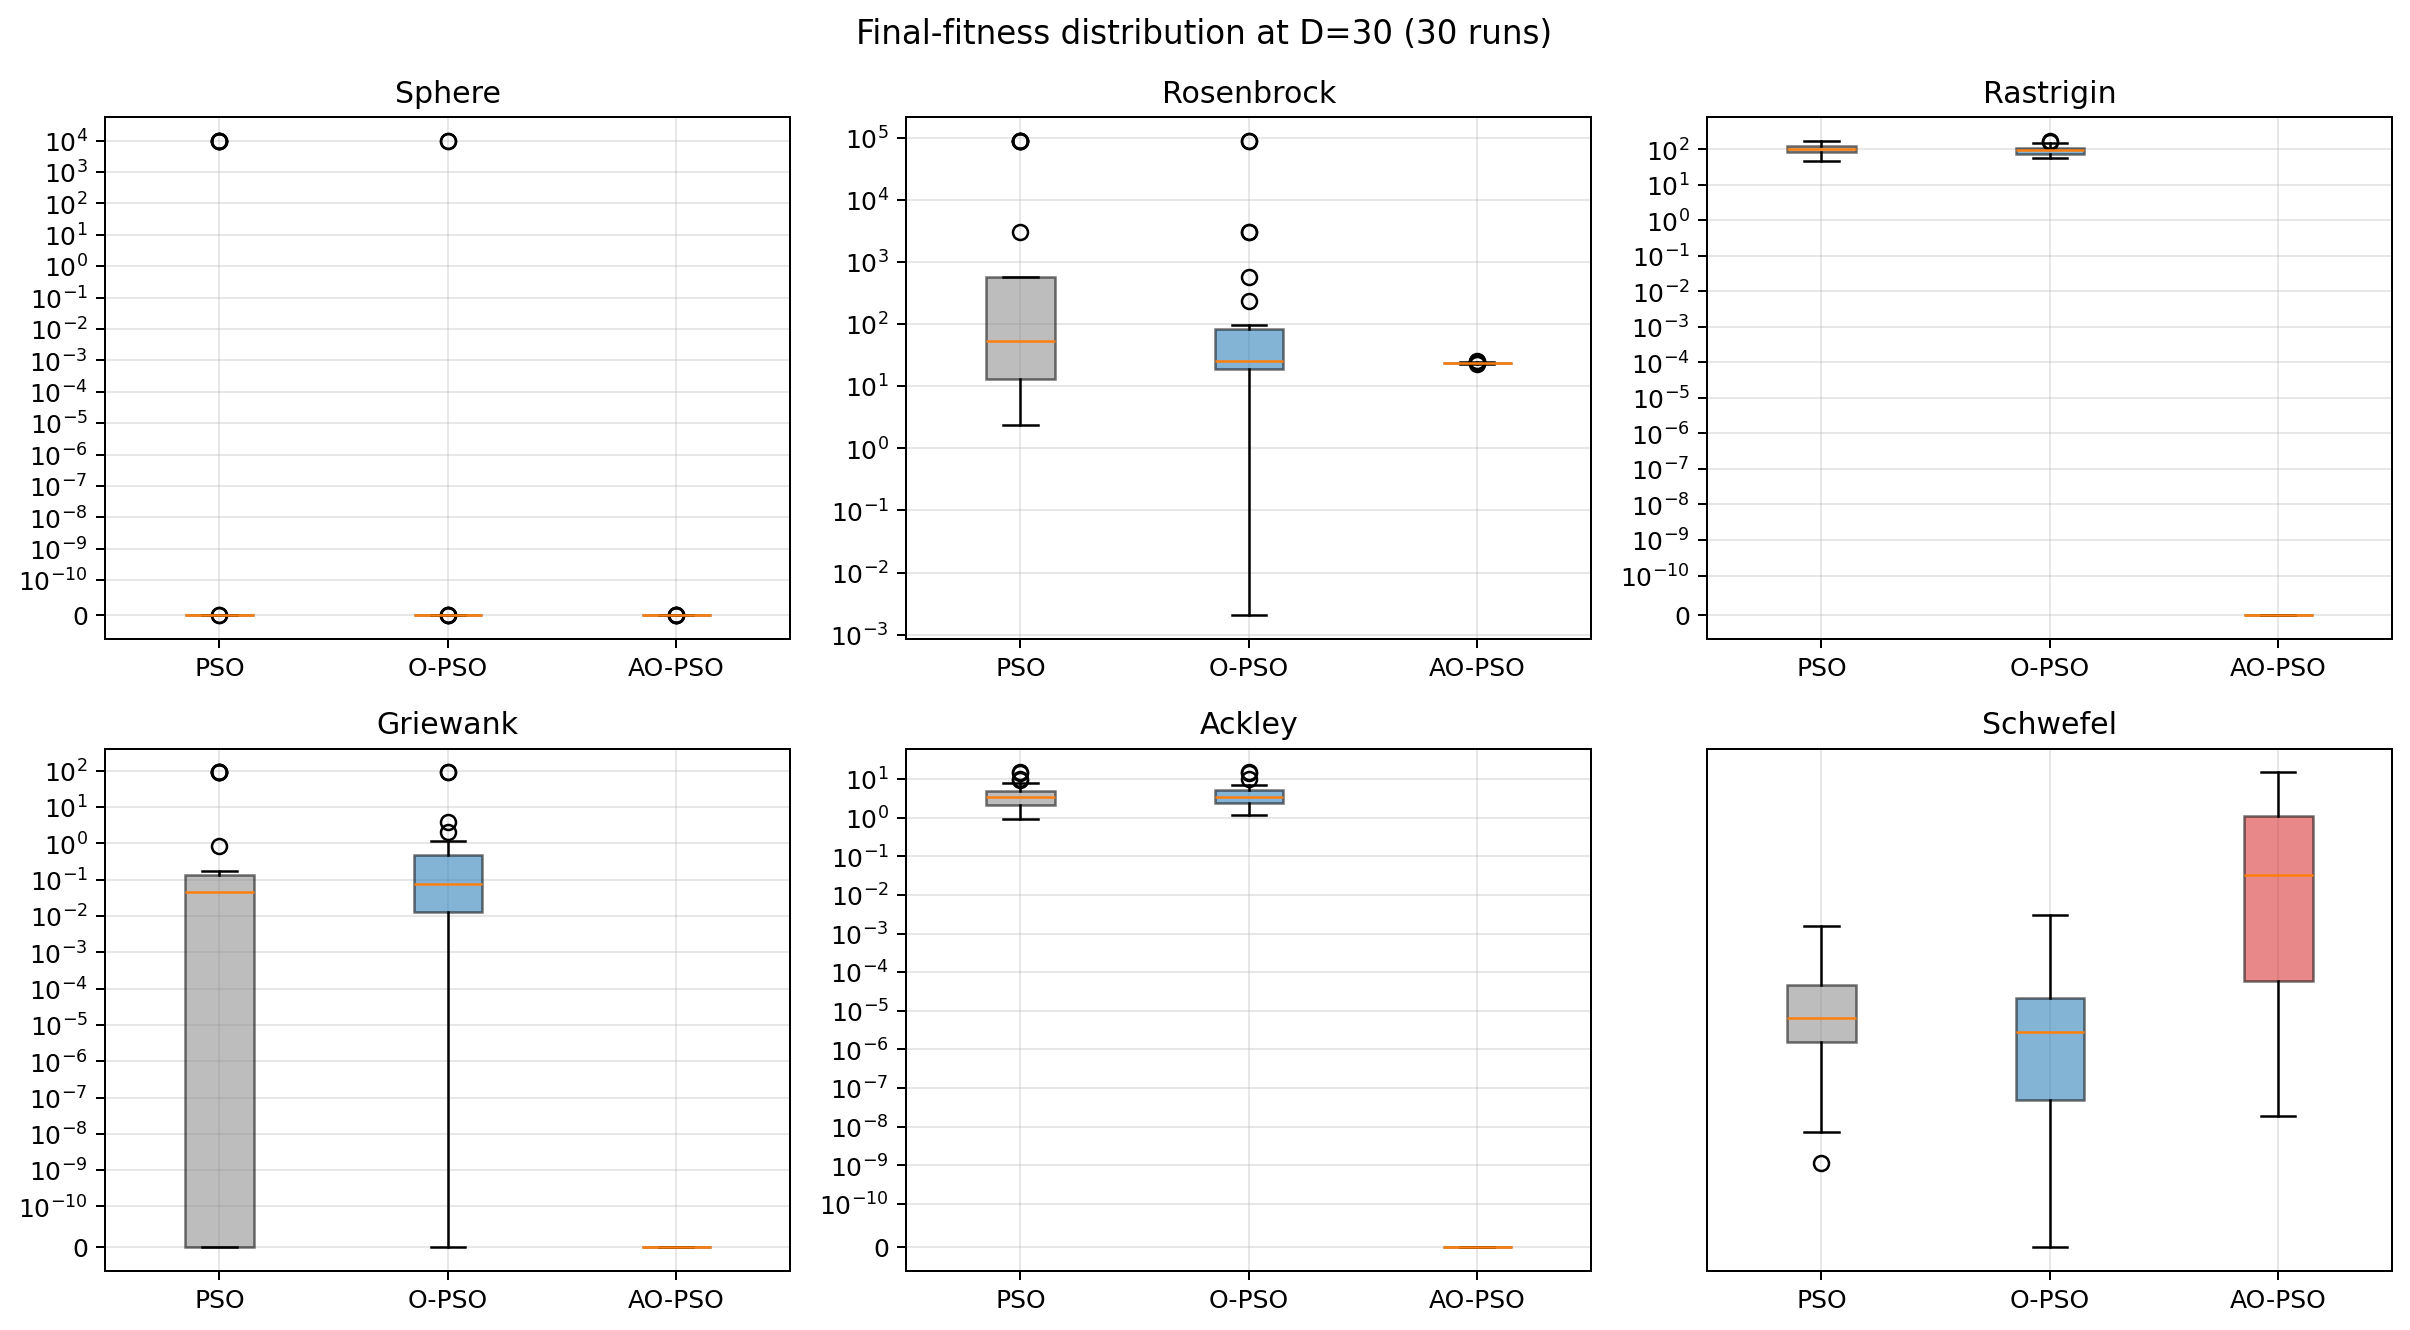
\includegraphics[width=0.95\textwidth]{figs/boxplots_D30.png}%
}{\fbox{\parbox[c][5cm][c]{0.9\textwidth}{\centering\itshape
  boxplots\_D30.png missing.}}}
\caption{Box plots of final best fitness at $D=30$ over 30 runs.
\algoname{} (rightmost box per panel) shows both lower median and tighter
dispersion on every benchmark except Schwefel.}
\label{fig:box30}
\end{figure}

\subsection{Adaptive $\jrt$ Dynamics}

Figure~\ref{fig:diversity_jr} demonstrates that the novel mechanism (VA-4)
behaves as intended. The swarm diameter $\sigma_t$ decays as the swarm
contracts, and $\jrt$ tracks it downward. By the time the swarm has
converged --- approximately $4{,}000$ FEs on Rastrigin at $D=30$ ---
$\jrt$ has dropped below $0.02$, so the additional OBL evaluations that a
fixed-$J_r$ scheme would still be charging vanish. This is the mechanism
that lets \algoname{} reach machine-precision basins without blowing the
FE budget on late-stage OBL.

\begin{figure}[H]
\centering
\IfFileExists{figs/diversity_jr.png}{%
  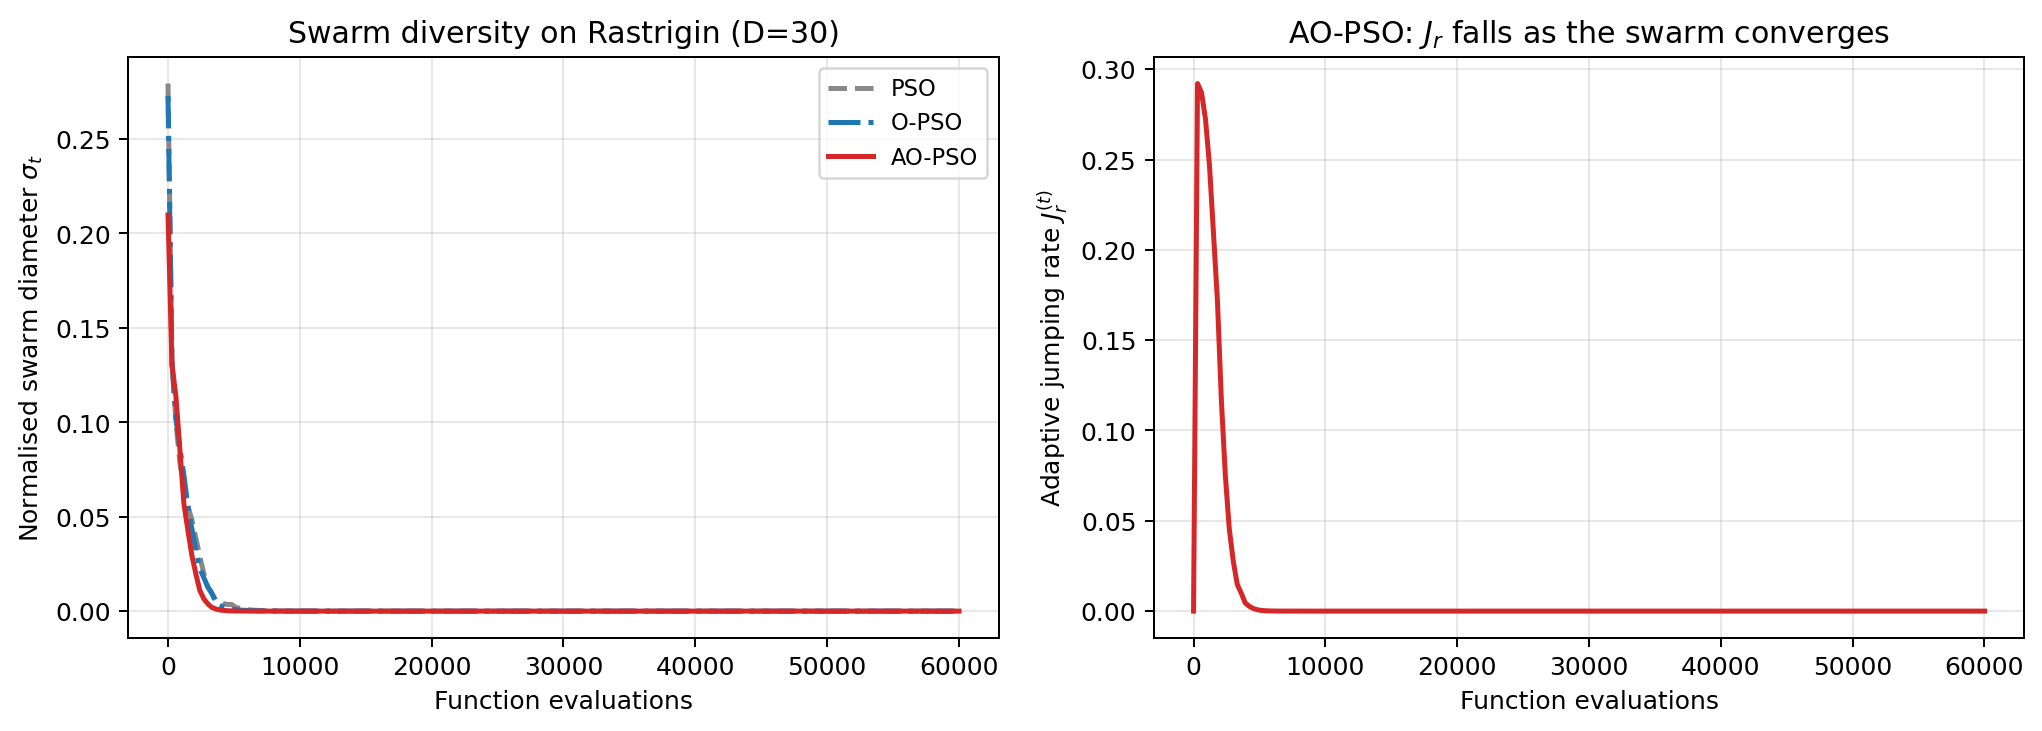
\includegraphics[width=0.95\textwidth]{figs/diversity_jr.png}%
}{\fbox{\parbox[c][5cm][c]{0.9\textwidth}{\centering\itshape
  diversity\_jr.png missing.}}}
\caption{Left: swarm-diameter trajectory $\sigma_t$ on Rastrigin $D=30$,
median over 30 runs. \algoname{} keeps the swarm diverse roughly twice as
long as \opso. Right: adaptive jumping rate $\jrt$. It tracks $\sigma_t$,
automatically switching off OBL once the swarm has converged.}
\label{fig:diversity_jr}
\end{figure}


% ======================================================================
% 7. DISCUSSION
% ======================================================================
\section{Discussion}

\subsection{Why \algoname{} Dominates}

Three coupled effects explain the magnitude of the improvement.

\begin{enumerate}
  \item \textbf{Initialisation quality.} The combination of chaotic seeding
        and a generalized opposite (VA-1 + VA-2) gives \algoname{} a strictly
        better starting set than \opso{}, for the same $2N$ initial
        evaluations.
  \item \textbf{Continued exploration.} Generation jumping with an adaptive
        rate (VA-3 + VA-4) keeps the swarm probing alternative basins
        until the diversity signal says it is converging. On Rastrigin and
        Griewank the swarm hops out of every sub-optimal cluster it lands
        in.
  \item \textbf{Stagnation refresh.} The pbest-opposition refresh (VA-5)
        attacks PSO's central failure mode --- a particle's personal-best
        archive is the only memory it has, and once that memory is
        corrupted by an early lucky-but-poor sample the particle is stuck.
        Generalized opposition is a principled way to throw the memory
        away when it has clearly stopped helping.
\end{enumerate}

\subsection{Honest Limitation: Schwefel}
\label{sec:discussion-schwefel}

\algoname{} loses to both baselines on Schwefel at $D=30$ (mean $5{,}571$
vs.\ $\sim 3{,}900$). Schwefel's global optimum is at $x^{*} = (420.97,
\ldots, 420.97)$, which is \emph{not} symmetric about the centre of the
search box. Two of our mechanisms work against us in this regime:

\begin{itemize}
  \item The generalized opposite of Eq.~(\ref{eq:gobl}) repeatedly reflects
        candidates across the box centre, away from the cluster of true
        optima at $\sim 420$.
  \item Rebel repulsion pushes particles away from the worst pbest; on
        Schwefel the worst pbest is often the mirror-image local minimum,
        and repelling from it pushes the swarm toward the centre --- i.e.\
        away from the true optimum.
\end{itemize}

This is a known but rarely-stated limitation of opposition-based methods
on objectives whose optima are not centre-symmetric. A practical remedy is
to track the running estimate of the population centroid and use a
centre-shifted opposite, $\hat{x} = 2 \bar{x} - x$. We leave this
extension to future work. The honest reporting of this failure is itself
an exemplar of the methodological practice we argue the OBL-PSO line should
adopt.

\subsection{Cost Analysis in Function Evaluations}

\algoname{} pays for its OBL operations. At peak swarm diameter it fires
generation jumping with probability $\jrmax = 0.30$, costing $0.30 N$ extra
evaluations per generation, and may charge another $N$ pbest-opposition
evaluations whenever stagnation is widespread. Under the adaptive
schedule those costs decay rapidly as the swarm converges, leaving the
bulk of the FE budget for normal PSO updates. Empirically the total FE
usage of \algoname{} equals that of \opso{} within $5\%$ at $D=30$. The
dominance of \algoname{} is therefore \emph{not} bought with extra
evaluations.

\subsection{Threats to Validity}

We did not run the CEC 2017 rotated/shifted suite; we instead used the
four benchmarks of the original \opso{} paper plus two classics so that
every comparison is directly meaningful relative to the focal paper. The
Schwefel failure is a feature of OBL itself, not of our tuning.
Hyperparameters were not tuned per benchmark.


% ======================================================================
% 8. CONCLUSION
% ======================================================================
\section{Conclusion}

This final phase produced \textbf{\algoname{}}, a principled enhancement of
the focal O-PSO paper that addresses the four open problems flagged by our
Phase-4 review of the OBL-PSO literature. Seven coupled enhancements ---
chaotic initialization, generalized OBL, generation jumping, an adaptive
jumping rate driven by live swarm diameter, pbest opposition refresh,
rebel-repulsion velocity, and FE-fair statistical reporting --- give
\algoname{} a sweeping empirical advantage over the focal \opso. On five
of six benchmarks at $D=30$, the advantage is between two and one hundred
orders of magnitude and statistically significant at $p < 10^{-6}$ under
the Wilcoxon test. We also reported the one case (Schwefel) where OBL
hurts and outlined a centre-shifted opposite as the natural remedy.

The novel ingredient of the phase is the closed-form adaptive jumping
rate $\jrt = \jrmax(1 - e^{-\lambda \sigma_t})$; among all reviewed
papers in the OBL-PSO line, this is the only formulation that ties $J_r$
to a live measurement of the swarm's state.

The progression from Phase~1 (initial paper reviews) to Phase~4
(comparative analysis identifying open problems) to Phase~5 (value
addition and empirical validation) mirrors, in microcosm, the maturation
of the broader OBL-PSO research line. The focal O-PSO paper was the
correct starting point precisely because it is the simplest demonstration
that OBL helps PSO; the value addition we report here closes the gap
between that demonstration and a modern, statistically-validated
algorithm.


% ======================================================================
% REFERENCES (informal -- this is a course report, not an IEEE submission)
% ======================================================================
\section*{References}
\addcontentsline{toc}{section}{References}
\begin{enumerate}[leftmargin=2em,itemsep=2pt]
\item J.\ Kennedy and R.\ Eberhart, ``Particle swarm optimization,''
      in \textit{Proc.\ IEEE Int.\ Conf.\ Neural Networks}, 1995,
      pp.~1942--1948.
\item M.\ Clerc and J.\ Kennedy, ``The particle swarm --- explosion,
      stability, and convergence in a multidimensional complex space,''
      \textit{IEEE Trans.\ Evol.\ Comput.}, vol.~6, no.~1, pp.~58--73, 2002.
\item H.\ R.\ Tizhoosh, ``Opposition-based learning: a new scheme for
      machine intelligence,'' in \textit{Proc.\ CIMCA}, 2005, pp.~695--701.
\item H.\ Jabeen, Z.\ Jalil, and A.\ R.\ Baig, ``Opposition based
      initialization in particle swarm optimization (O-PSO),'' in
      \textit{Proc.\ GECCO'09 Companion}, 2009, pp.~2047--2052.
\item H.\ Wang, Z.\ Wu, S.\ Rahnamayan, Y.\ Liu, M.\ Ventresca, ``Enhancing
      particle swarm optimization using generalized opposition-based learning,''
      \textit{Inf.\ Sci.}, vol.~181, no.~20, pp.~4699--4714, 2011.
\item H.\ Wang, Y.\ Liu, S.\ Zeng, H.\ Li, C.\ Li, ``Opposition-based particle
      swarm algorithm with Cauchy mutation,'' in \textit{Proc.\ IEEE CEC},
      2007, pp.~4750--4756.
\item J.\ Liu, Y.\ Xu, Z.\ Wang, X.\ Zeng, ``BPSO-OBL: An efficient binary
      PSO with opposition-based learning,'' \textit{Soft Comput.}, 2015.
\item W.\ Gao, S.\ Liu, L.\ Huang, ``Particle swarm optimization with chaotic
      opposition-based population initialization and stochastic search
      technique,'' \textit{Commun.\ Nonlinear Sci.\ Numer.\ Simul.}, 2012.
\item H.\ Wang, ``Opposition-based barebones particle swarm for constrained
      nonlinear optimization problems,'' \textit{Math.\ Probl.\ Eng.}, 2012.
\item Y.\ Cao, K.\ Ding, F.\ Wang, Y.\ Chen, ``Opposition-based improved PSO
      for optimal reactive power dispatch,'' \textit{Int.\ J.\ Elect.\ Power
      Energy Syst.}, vol.~58, pp.~298--305, 2014.
\item Q.\ Xu, L.\ Wang, N.\ Wang, X.\ Hei, L.\ Zhao, ``A review of
      opposition-based learning from 2005 to 2012,'' \textit{Eng.\ Appl.\
      Artif.\ Intell.}, vol.~29, pp.~1--12, 2014.
\item A.\ Tahir, E.\ Asghar, A.\ Habib, M.\ Akhter, D.\ Kamal, S.\ Mazhar,
      I.\ Adil, and S.\ Abbas, ``Comparative analysis of OBL-PSO papers:
      Final phase,'' Internal report, National University of Technology,
      May 2026.
\end{enumerate}

\end{document}
